
\section{Control} \label{section:control}
Control is an essential aspect of any generative model. Without control, even the best generative models producing beautiful music would be of very limited real-world use. Control allows generative AI tools to become proper collaborative systems, and generate for a wide array of scenarios. In music generation control covers essentially all musical parameters. Parameters vary by representation, symbolic music for instance leaves very little room for any type of timbre control (aside from instrument selection). 
“Raw” audio models such as Stable Audio (Evans et al., 2024) can for instance be controlled for acoustic settings (i.e jazz music playing in a busy restaurant, in a \textit{large cathedral}, or \textit{through an intercom}), something that is simply not represented in symbolic music. 
For musical parameters represented in symbolic music, there are different approaches to classifying them. 
One can differentiate between global and local features (discussed in the appendix \ref{feature_cat}) \cite{Van_Kranenburg_Volk_Wiering_2013}, 
deep vs surface-level features \cite{Blacking_1971}, high-level vs low-level features \cite{Tan_Herremans_2020} and global vs fine-grained or time-varying features. 

In the context of this thesis we differentiate between global features, and time-varying features \cite{Rütte_figaro_2023}. What is time-varying or global is highly context dependent, a piece may have one time-signature and tempo as is assumed in \cite{Lu_Xu_Kang_Yu_Xing_Tan_Bian_MuseCoco_2023} or it may vary over time as is suggested in \cite{Rütte_figaro_2023} or \cite{Huang_Yang_remi_pop_transformer_2020}. Other time varying controls could be chords \cite{Rütte_figaro_2023}\cite{Wu_Donahue_musicontrolnet_2023}\cite{Lan_Hsiao_Cheng_Yang_musicongen_2024}\cite{Min_Jiang_Xia_Zhao_polyffusion_2023}, melody \cite{copet2023simple}\cite{Min_Jiang_Xia_Zhao_polyffusion_2023} or texture \cite{Min_Jiang_Xia_Zhao_polyffusion_2023}. For the target application in an MACT - game, time-varying controls are necessary to provide a change in music that triggers a change in the patients improvisation.


\subsection{Rhythmic control} \label{section:rhytmic_weight}
The types of control exercised over rhythmic components varies by representation as discussed in \ref{representation}. In CocoMulla \cite{Lin_cocomulla_2024} generated audio is controlled with drum tracks and a piano-roll. Similarly in JASCO\cite{Tal_jasco} drum-audio is used for conditioning. In MusicConGen.\cite{Lan_Hsiao_Cheng_Yang_musicongen_2024}control for rhythm is added through tracking beats and downbeat. MusicControlNet\cite{Wu_Donahue_musicontrolnet_2023} adds beat and downbeat conditioning to an audio diffusion model.
For symbolic systems control of tempo and meter is relatively common \cite{Rütte_figaro_2023}, \cite{Huang_Yang_remi_pop_transformer_2020}, \cite{Lu_Xu_Kang_Yu_Xing_Tan_Bian_MuseCoco_2023}. Time-varying control over rhythm is often deployed through note-density (both vertical and horizontal)\cite{Rütte_figaro_2023},\cite{Huang_rule_diffusion_2024}. Another approach \cite{Zhu_Liu_Jiang_Zheng_texture_2024} involves passing the piano-roll as factor to guide the diffusion process. In Polyffusion\cite{Min_Jiang_Xia_Zhao_polyffusion_2023} Min et al successfully encode texture, that is disentangled into harmony and rhythm using a pre-trained variational auto-encoder \cite{Wang_vae_chord_rhythm_2020}. Herremans et al \cite{Tan_Herremans_2020} control rhythm through the high-level feature arousal, that is disentagled using a variational autoencoder into rhythm and note-density. 


\subsection{Inner Metric Analysis} 
Using a variational auto-encoder to disentangle rhythmic descriptions into lower level features is an option, but introduces additonal complexity of training a second model, and combining both to be used for inference. Instead, we use Inner Metric Analysis (IMA) to create metric profiles of a sequence, and use theese profiles as guiding features. Inner Metric Analysis identifies strong and week pulses and their periods within note onset in symbolic music.\cite{} It is used to identify \textit{local meters} as opposed to \textit{outer meter} given by time-signatures, which can be useful in the study of syncopation \cite{Bemman2024}\cite{Volk2008Syncopation}. IMA is also used in the classification of dance-music \cite{Chew_Volk_Lee_Dance_metric_weight_2005}, automatic detection of meter \cite{Haas_Volk_2016} and music retrieval \cite{Volk_Garbers_VanKranenburg_Wiering_Grijp_Veltkamp_2009}. 

A local meter is a set of evenly spaced onsets with a minimum length of three, not able to be extended forward or backwards in time, and not contained within any other local meter. (see figure \ref{fig:ima_all}). Let $M(l)$ be the set of local meters with a length of at least l. The parameter $p$ is variable and determines how much the length of a local meter influences its weight. Intuitivly, longer and more established local meters should carry more weight. This is given by $k_{m}^p$. The weight of an onset $W_{l,p}(o)$ is defined as the weighted sum of the local meters.  
The metric weight is calculated as follows \cite{Volk2008Syncopation}.  

\begin{equation}
    W_{l,p}(o) = \sum_{m \in M(l):o \in m}k_{m}^{p}
\end{equation} 
Spectral weight is a variation of the metric weight, that consider the extension of each local meter: $ext(m)$. The red triangles in figure \ref{fig:ima_all} are and example of extensions. The calculation is similar, but it assigns a weight to each time point (instead of only to onsets) and considers the extensions. This feature is less sensitive to local changes.

\begin{equation}
    SW_{l,p}(t) = \sum_{m \in M(l):t \in ext(m)}k_{m}^{p}
\end{equation}

In the context of MACT, inner metric analysis is interesting because it can indicate rhythmic complexity, which in turn can influence ease of tapping along \cite{Volk2008Syncopation} and rhythmic entrainment. This could be extended to generate music that is more difficult to follow to allow for difficulty adjustment in the context of an MACT game. 

\begin{figure}[H]
    \centering
    \begin{subfigure}{0.45\textwidth}
        \centering
        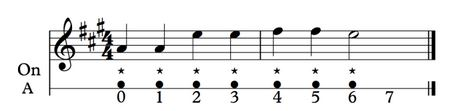
\includegraphics[width=\linewidth]{IMAGES/IMA1.JPG}
        \caption{Single local meter and its pulses (A) from the melody "Twinkle, Twinkle Little Star"}
        \label{fig:ima1}
    \end{subfigure}
    \begin{subfigure}{0.45\textwidth}
        \centering
        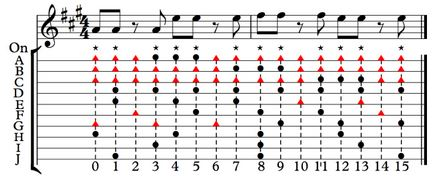
\includegraphics[width=\linewidth]{IMAGES/IMA2.JPG}
        \caption{10 local meters and their pulses produced by IMA of a syncopated variation of "Twinkle, Twinkle Little Star"}
        \label{fig:ima2}
    \end{subfigure}
    
    \vspace{0.5cm} % Adjust spacing between rows

    \begin{subfigure}{0.45\textwidth}
        \centering
        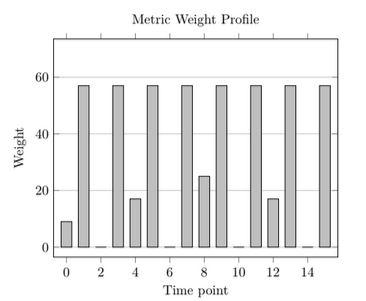
\includegraphics[width=\linewidth]{IMAGES/IMA3.JPG}
        \caption{Metric weight profile of syncopated "Twinkle, Twinkle Little Star"}
        \label{fig:ima3}
    \end{subfigure}
    \begin{subfigure}{0.45\textwidth}
        \centering
        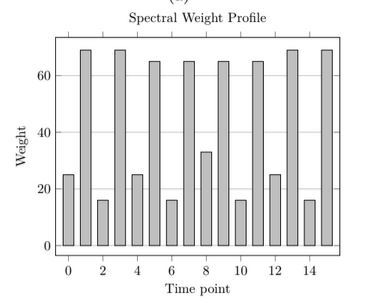
\includegraphics[width=\linewidth]{IMAGES/IMA4.JPG}
        \caption{Spectral weight profile of syncopated "Twinkle, Twinkle Little Star"}
        \label{fig:ima4}
    \end{subfigure}

    \caption{Visualisation of metric weight analysis \cite{Bemman2024}}
    \label{fig:ima_all}
\end{figure}


\section{Implementation of control} \label{section:addingcontrol}
Adding control to generative models can be split into three approaches. 1: Choice of architecture and training data, 2: fine-tuning approaches, and 3: external conditioning or guidance.

\subsection{Control through architecture}
The choice of architecture lends itself to different types of control. Transformers are next token predictors, that predict based on the prior sequence. The default training paradigm allows for conditioning with a user defined musical (or audio) sequence. This is true for both audio based models such as MusicGen \cite{copet2023simple}, Jukebox \cite{Dhariwal_Jun_Payne_Kim_Radford_Sutskever_2020} and MusicLM \cite{Agostinelli_Denk_Borsos_Engel_Verzetti_Caillon_Huang_Jansen_Roberts_Tagliasacchi_et_al._2023} as well as symbolic music models such as MMT \cite{Dong_Chen_MMT_Kirkpatrick_2023}, MusicTransformer \cite{Huang_Vaswani_Uszkoreit_Shazeer_Simon_Hawthorne_Dai_Hoffman_Dinculescu_Eck_2018} and MusicBERT \cite{Zeng_Tan_Wang_MUSICBERT_2021}. 

Diffusion models are quite flexible compared to transformers, the same model can be used for inpainting, continuation and depending on the representation melody and accompaniment generation through masking.\cite{Min_Jiang_Xia_Zhao_polyffusion_2023}\cite{Rombach_Blattmann_Lorenz_Esser_Ommer_2022}

\subsection{Control through training conditioning}
Control can be added through training data. MusicGen\cite{copet2023simple}, a recent text-to-music (audio) transformer is trained on 20000 hours of licensed music from shutterstock and pond5 \footnote{https://www.shutterstock.com/music and https://www.pond5.com/} which includes textual descriptions and tags for genre, tempo, and other factors such as instrumentation. Control is achieved through the joint training of a text description and music. An example description is provided below: 

\textit{Inspirational dramatic background music! Perfect for trailer, background, advertising, historical film, movie about superheroes, teaser and many other projects!}\footnote{ https://www.pond5.com/royalty-free-music/item/95908062-inspiring-dramatic-epic-background-cinematic-music
}

Text-based control, while user-friendly and accessible to non-musicians, is inherently vague. Levels of detail and choice of words vary widely by dataset, even with standardized tags such as genre and tempo. Specialized datasets such as MusicCaps \cite{Agostinelli_Denk_Borsos_Engel_Verzetti_Caillon_Huang_Jansen_Roberts_Tagliasacchi_et_al._2023}, which contains 5500 text music pairs, with 10 seconds of music alongside a free text description and a list of aspect tags created by human experts still suffer substantially from subjectivity \cite{Lee_Doh_Jeong_2023_subjectivity_musiccaps}. 

For this reason, the creators of MusicGen \cite{copet2023simple} add melody conditioning alongside text conditioning and train their model jointly with the chromagram of the melody alongside the text.

In MusicGenStyle \cite{Rouard_Adi_Copet_Roebel_Défossez_musicgenstyle_2024} perform classifier-free guidance to add style conditioning to MusicGen. They train a music-style encoder that transforms a random subsample of a given reference audio track into tokens that are combined with the embeddings of the text-description. Both the style tokens and text tokens are provided as prefix to the model. The conditioner and the MusicGen transformer are trained jointly on the entire dataset. 

The creators of FIGARO\cite{Rütte_figaro_2023} enable fine grained control over instrumentation, note density, average pitch and volume on a bar-by-bar basis, in a symbolic music generator through joint conditioning while training. 

\subsection{Adding control through fine-tuning}

Both the melody conditioning of MusicGen \cite{copet2023simple} and the style conditioning of MusicGenStyle \cite{Rouard_Adi_Copet_Roebel_Défossez_musicgenstyle_2024} retrain the entire MusicGen model on the entire dataset which comes at considerable cost. Fine-tuning or transfer learning is another method through which models can be trained but at considerably smaller cost and using less data. This is particularly useful and widely used in the language domain to adjust large language models for niche use-cases, where the available data may simply not be sufficient to train a large model from scratch. In the examples of MusicGen and MusicGenStyle the availability of data was not a limiting factor since the controlling elements, melody and style can be inferred from the training data. However fine-tuning is also helpful for adding new control mechanisms.

MusiConGen \cite{Lan_Hsiao_Cheng_Yang_musicongen_2024} is a fine-tuned variation of MusicGen which adds rhythm and chord control. They propose the jump-finetuning mechanism, where the original model with 1.5 Billion parameters and 48 self-attention layers, is split model into blocks consisting of 4 self-attention layers. They refine the first layer of each block, freezing the remaining layers. Additionally, they apply adaptive in-attention to the first 9 blocks, where the output of the transformer is augmented with copies of the original condition. As a result, only a quarter of the original parameters are tunable, which enables training on consumer GPUs on just 250 hours of music sourced from YouTube (as opposed to 20000 hours).  In Coco-Mula \cite{Lin_cocomulla_2024} the authors adjust a LLAMA adapter with just 4\% of parameters, keeping all original MusicGen parameters frozen, and training only the adapter on a small dataset of 300 songs to add drum and chord conditioning. 

MuseBarControl \cite{Shu_Xu_Musebarcontrol_2024} is a fine-tuned version of MuseCoco\cite{Lu_Xu_Kang_Yu_Xing_Tan_Bian_MuseCoco_2023} which extends the global controls with time-varying bar level control for music-generation. They compare several approaches. In the first they augment the prompt (which is generated from text) with additional tokens for bar-wise control of chords, and adjust the loss function to incoperate that.  In the second approach they introduce two novel methods, first, they pre-adapt the new parameters (introduced by the lora adapter) to a separate classification task, an auxiliary task . The model classifies whether the a section of music corresponds with the control tokens, the body of the model is trained together with a classification head (which is removed after auxiliary task training. In the third step they introduce counterfactual loss where the difference in negative log likelyhood conditioned on the original and changed attribute is maximized, which reinforces the models attention to the control. They find that the combination of the three strategies, pre-adaptation on a separate task followed with counterfactual-loss and prompt augmentation yields the strongest model. 

\subsection{Adding control through guidance}
There are also other methods that do not involve any finetuning or retraining of the original model. Adding control through rule labels, or control tokens as in \cite{Rütte_figaro_2023}\cite{Lan_Hsiao_Cheng_Yang_musicongen_2024} does require some amount  retraining, which is not always feasible, and adding many different types of control may deterioate the model. In these cases, guidance can be used to steer the model towards a certain output.
In SMITIN \cite{Koo_Wichern_Germain_SMITIN_2024} the authors use inference time intervention to guide a model towards a certain output with respect to certain goals. The goals explored are the presence of certain instruments (piano/drums/bass/guitar) in the mix and the quality/realism of the music. The authors train linear probes that learn to associate a state of the attention heads with the stated goal. Then the attention heads are steered in the direction of the probe’s output, which increases the probability of the desired quality being present in the generated music.   

In Diffusion models, the output is sampled over several steps, at each of these steps it is possible to intervene with guidance to direct the sampling towards a certain goal. In \cite{Huang_rule_diffusion_2024}, each sampling step is repeated several times, and each time the sample that follows a set of rules most closely is chosen. ControlNet \cite{Zhang_Rao_Agrawala_2023} adds spacial control to image generators allowing the guidance of image generation using sketches, poses, edges and depth maps without retraining. MusicControlNet \cite{musicwellbeing_agres_2021} adapts this approach to music generation adding control for time varying factors, melody, dynamics and rhythm. 


\section{Evaluation} \label{section:evaluation}
How to evaluate generated music is still an open research question. There are no standardized methods according to which evaluations happen\cite{Yin_Reuben_Stepney_Collins_2023}. In the context of music generation there are several proposed frameworks to evaluate music. Typically we differentiate between subjective and objective evaluations.

For subjective approaches the methods vary widely \cite{Xiong_Wang_ai_eval_methods_2023}. There are simple Turing-type evaluations that test how distinguishable generated and human written music are. Then there are subjective query metrics, where typically likert ratings of different parameters are collected.\cite{Min_Jiang_Xia_Zhao_polyffusion_2023}.
There are tournament style surveys, where the number of winning pieces are tallied for each approach.\cite{Huang_Vaswani_Uszkoreit_Shazeer_Simon_Hawthorne_Dai_Hoffman_Dinculescu_Eck_2018}\cite{Rütte_figaro_2023} Finally there are expert evaluations (which can also include likert ratings) but also analysis of the produced score and musical structure. \cite{Sturm_Ben-Tal_2016} These evaluations are often paired with statistical hypothesis testing. \cite{Rütte_figaro_2023}\\

Automatic evaluation of generated music include model specific metrics and different musical metrics \cite{Xiong_Wang_ai_eval_methods_2023}. Model specific metrics are generic evaluations of a models success to approximate training data, these will vary depending on the model and are not indicative of stylistic success. Examples of this are Negative Log Likelyhood \cite{Huang_Vaswani_Uszkoreit_Shazeer_Simon_Hawthorne_Dai_Hoffman_Dinculescu_Eck_2018}, Root Mean Square Error \cite{Rütte_figaro_2023} or Perplexity\cite{Rütte_figaro_2023}. Musical metrics typically involve comparing a set of generated music to a set of real music, there are plenty of musical similarity measure techniques\cite{Gurjar_Moon_similarity_2018} for a large variety of different use-cases i.e music retrieval, cover, genre and artist detection. A popular comparative metric is calculating the Kulback Leibler (KL) divergence between two datasets with respect to certain metrics i.e count of intervals or unique pitch-classes. However to obtain the divergence one has to select specific features that may only capture a subset of the desired properties. Similar issues arise with other distance metrics i.e cosine similarity, earth movers distance or maximum overlapping area. 

Especially in the audio domain, additional AI models are often used for evaluation. MusicGen \cite{copet2023simple} uses additional classifiers to generate labels for the music and calculates the KL-divergence between the generated labels. Additionally they calculate the Frachet Audio distance, a measure devised to calculate the plausibility of audio (for music enhancement purposes) compared to a large set of studio recordings\cite{Kilgour_Frachet_2019}. Finally they use the CLAP-score which compares the corresponding text description to the latent representation of the generated audio, with text-description of the generated audio with the reference audio. \cite{Elizalde_Deshmukh_Ismail_Wang_2023}

For this thesis we are interested in two factors, first the plausibility of the generated music, and second the success of the control. How the success of control is evaluated depends on what is controlled for,  Examples of controlled parameters and how they are evaluated are as follows:

\textbf{Note Density}.  (how many notes per bar). Root mean square error (RME) between generated vs target notes per bar. This is the approach to compare note density used in \cite{Rütte_figaro_2023}

\textbf{Note Variability} (number of unique pitch classes, normalized by number onsets) - RME between generated and target.

\textbf{Rhythmic patterns}. Partial Similarity \cite{Volk_Garbers_VanKranenburg_Wiering_Grijp_Veltkamp_2009} between target and generated music: 

Evaluating the plausibility of generated music is more complex, and there is no one method that has been proven superior. Possibly the plausibility of the music will be evaluated with a (small) subjective study. In this scenariou we would follow \cite{Dong_Chen_MMT_Kirkpatrick_2023}, \cite{Yu_Lu_Wang_Hu_Tan_Ye_Zhang_museformer_2022} and \cite{Chen_Smith_Spijkervet_Wang_Zou_Li_Kong_Du_2024} and collect likert ratings on questions targeting Coherence Richness Arrangement and Consistency . Theese are would be paired with questions on musical background and preferences of the participant. 
For objective rating of the plausibility of the music we will follow the approach by \cite{Min_Jiang_Xia_Zhao_polyffusion_2023} where the KL-divergence between the corpus of generated and a corpus of original music is calculated, most likely KL divergence over a set of extracted features, such as a pitch classes and chords. For a more complete list of different evaluation methods used on symbolic music generators, refer to the notes in the abstract \ref{section:compare_sym}.
